\chapter{Project Management}


\section{Planning}\label{sec:planning}

\begin{table}[H]
    \begin{tabularx}{\textwidth}{ l X l }
        \hline
        \textbf{\textnumero} & \textbf{Milestone}                     & \textbf{Date of Achieval} \\ \hline
        MS\_1                & Cultivation of Bacteria                & 09.11.2023                \\
        MS\_2                & Extraction of LanM                     & 07.12.2023                \\
        MS\_3                & Detection of LanM                      & 14.03.2024                \\
        MS\_4                & Binding of LanM to Rare Earth Elements & 29.02.2024                \\
        MS\_5                & Separation of Rare Earths from LanM    & not confirmed yet         \\
        \hline
    \end{tabularx}
    \caption{Planned milestones and their date of achieval.}
    \label{tab:milestones}
\end{table}


\section{Evaluation\authorA{}}

\begin{figure}[H]
    \centering
    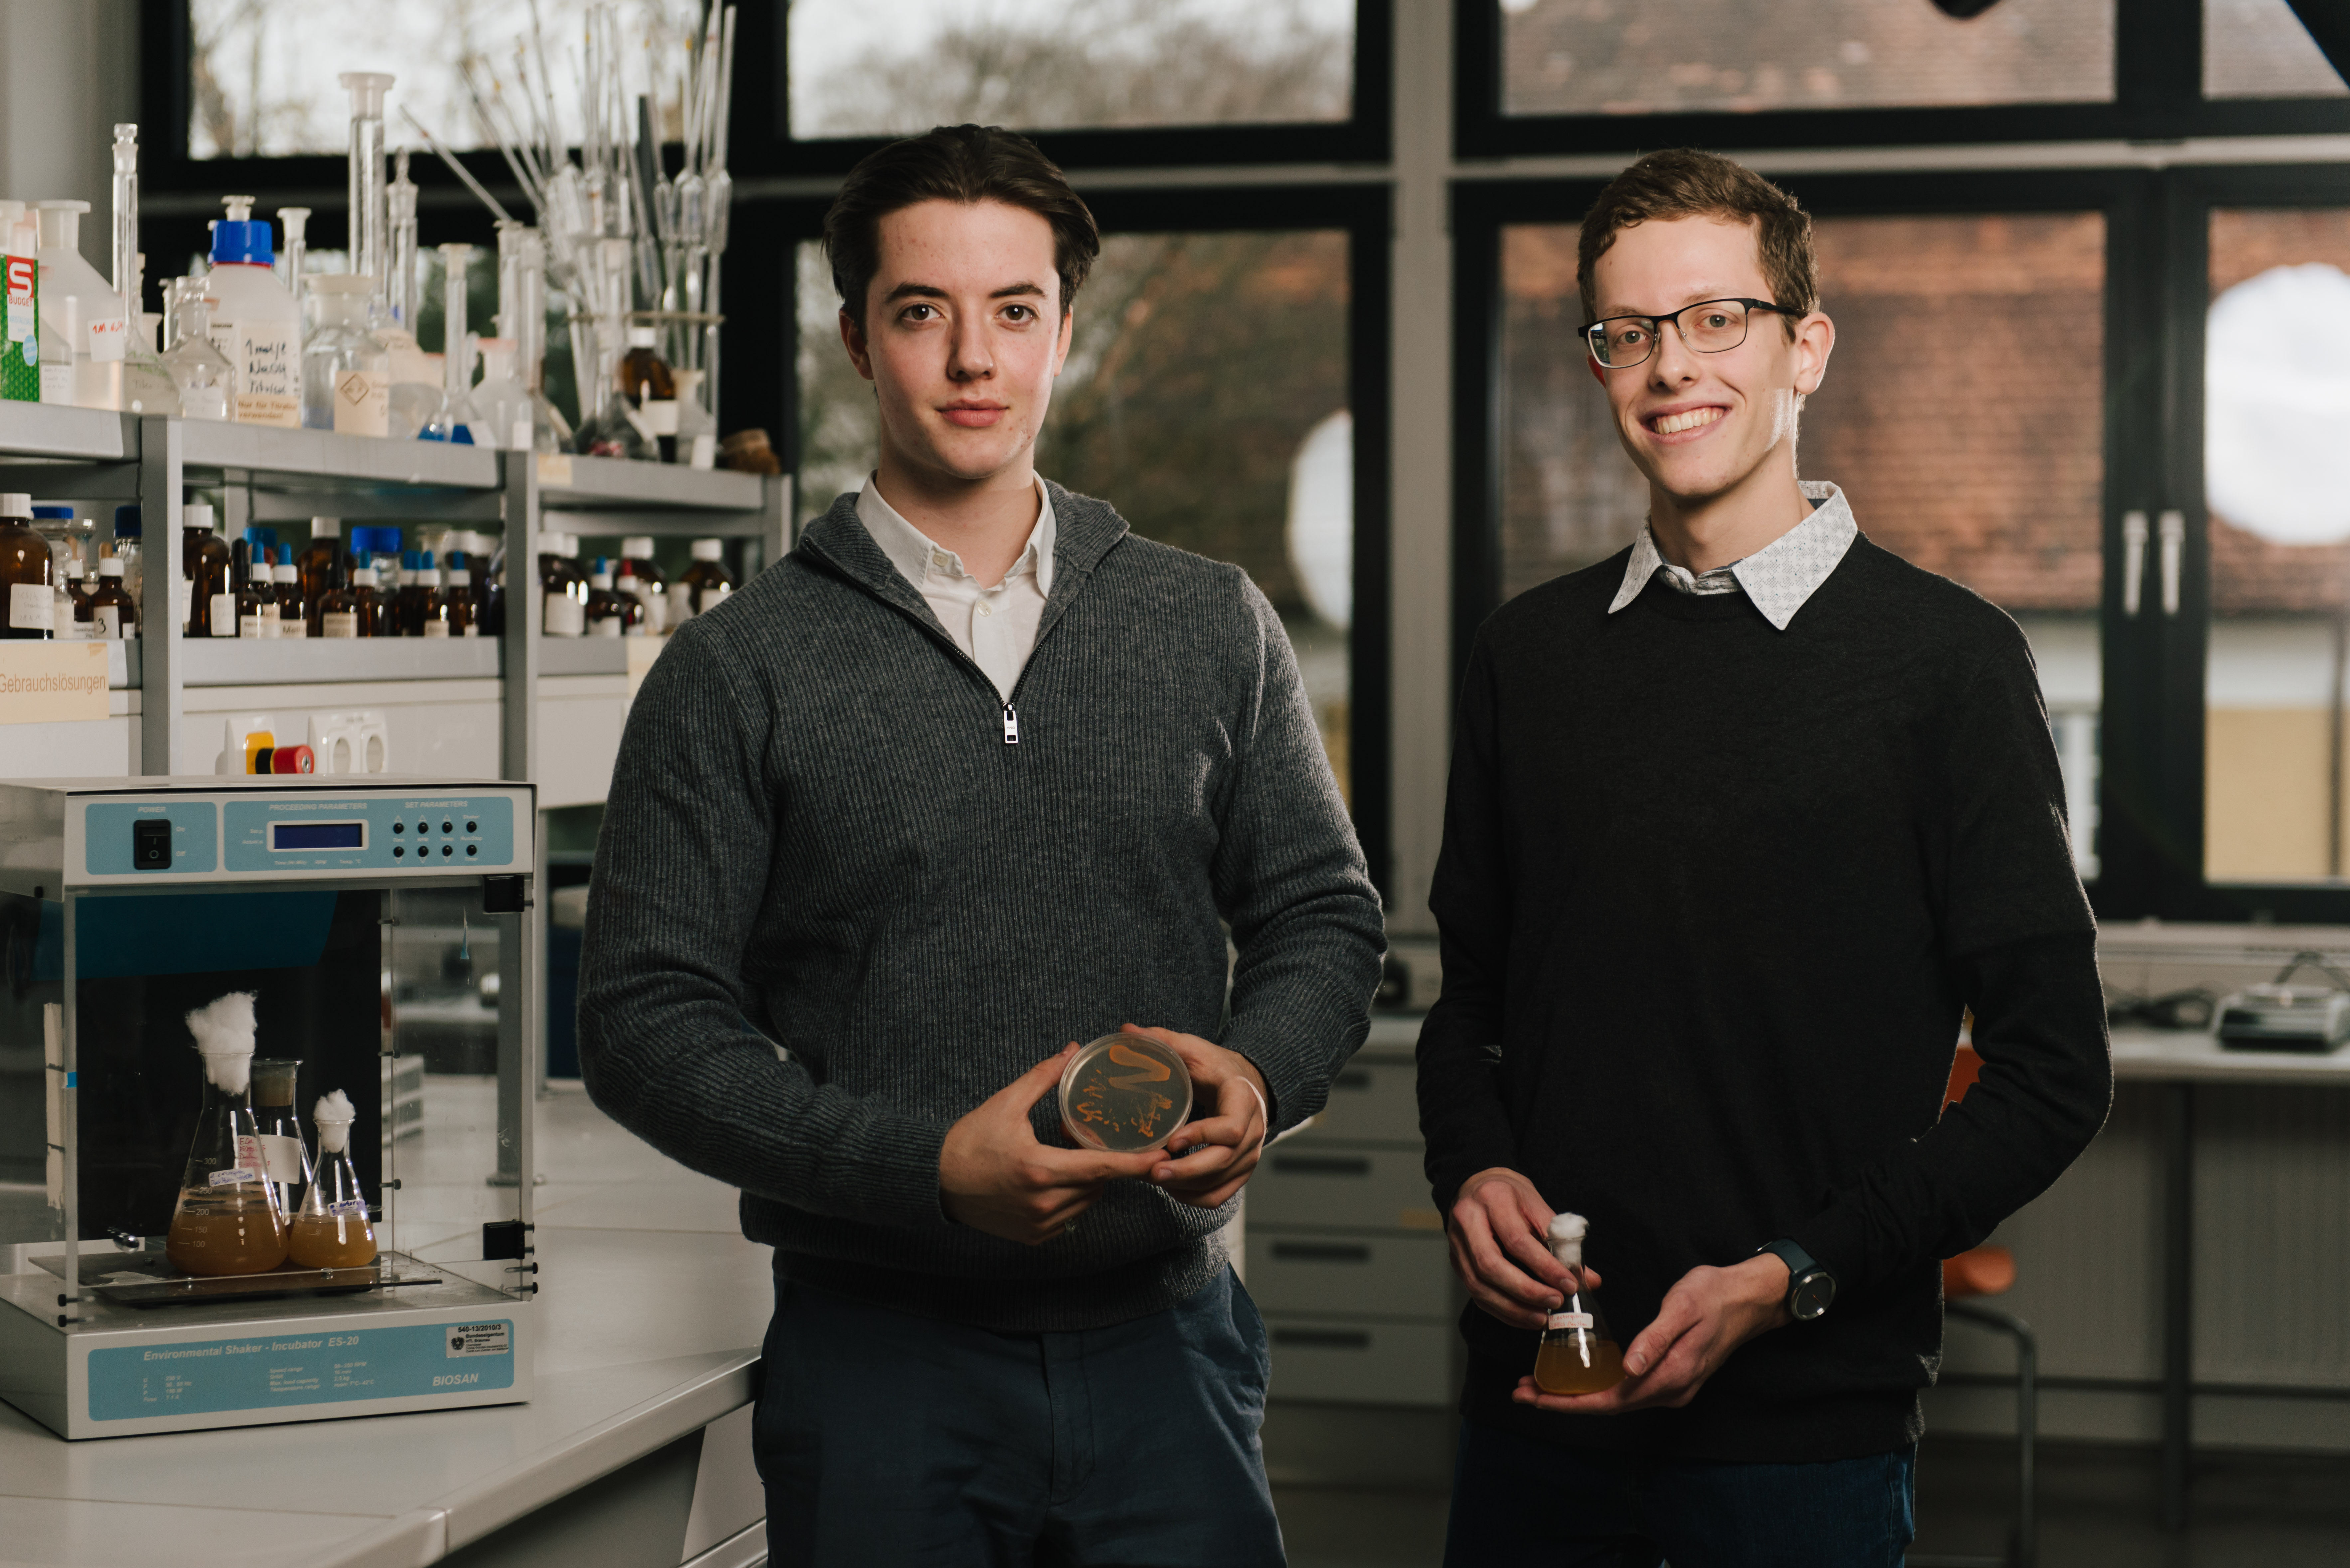
\includegraphics[width=0.8\textwidth]{./media/images/Gruppenfoto}
    \caption{The project team}
    \label{fig:teamphoto}
\end{figure}

When we started to conduct some research for the project in the summer break, we also simultaneously began to plan the work with agile project management methods.
As it turned out, doing the project management this way was really helpful.
During our work, we encountered a lot of obstacles which we had not thought of before, which resulted in a slower progress than we had previously expected.

Another problem that we encountered was that we simply could not do our project the way we had planned at the beginning.
Due to limited financial resources and equipment, we could not carry out our planned work.
A lot of methods we tried out did not produce the expected or reliable results.
When we ran into these problems, we had to change how we want to achieve our planned goals.
This also meant that one of our planned milestones (MS\_3 Detection of LanM, see table~\ref{tab:milestones} in section~\ref{sec:planning}) was achieved later and also in a different way than we initially expected.

After we had tried our new approach, we finally achieved promising results.
This brought fresh air into the project because we saw that progress was being made.
After weeks of repeated failure, we found new motivation to keep going.

Our new approach requires less expensive resources and is simpler to carry out.
Overall, this made our project better, and it did not change our main goal.
The transformation from our first approach to the other would not have been possible if we had not used agile project management methods.



\newpage


\section{Timesheet}

\subsection{Tobias Daxecker}

\begin{longtable}{|c|p{7cm}|c|c|}
    \hline
    \textbf{Date} & \textbf{Work}                                                                                                   & \textbf{School Time} & \textbf{Free Time} \\ \endhead \hline
    03.08.2023    & Research                                                                                                        & 0,00                 & 3,00              \\ \hline
    18.08.2023    & Research                                                                                                        & 0,00                 & 2,00              \\ \hline
    24.08.2023    & Research                                                                                                        & 0,00                 & 2,00              \\ \hline
    03.09.2023    & Research                                                                                                        & 0,00                 & 1,00              \\ \hline
    06.09.2023    & Research                                                                                                        & 0,00                 & 2,00              \\ \hline
    07.09.2023    & Research                                                                                                        & 0,00                 & 4,00              \\ \hline
    08.09.2023    & Preparation of nutrient solution                                                                                & 0,00                 & 6,00              \\ \hline
    14.09.2023    & Cerium detection                                                                                                & 10,00                & 0,00              \\ \hline
    21.09.2023    & Production of solid culture medium                                                                              & 10,00                & 0,00              \\ \hline
    22.09.2023    & Organization of teams                                                                                           & 0,00                 & 1,00              \\ \hline
    28.09.2023    & Profile, milestones                                                                                             & 0,00                 & 1,00              \\ \hline
    02.10.2023    & Research                                                                                                        & 0,00                 & 1,00              \\ \hline
    05.10.2023    & Preparation of nutrient solution, detection of rare earths                                                      & 10,00                & 0,00              \\ \hline
    06.10.2023    & Freezing the bacteria                                                                                           & 0,00                 & 1,00              \\ \hline
    09.10.2023    & Research                                                                                                        & 0,00                 & 1,00              \\ \hline
    10.10.2023    & Research, research plan                                                                                         & 0,00                 & 2,00              \\ \hline
    12.10.2023    & Cultivation of M. extorquens, preparation of SDS-PAGE                                                           & 10,00                & 0,00              \\ \hline
    15.10.2023    & Draft research plan                                                                                             & 0,00                 & 3,00              \\ \hline
    16.10.2023    & Draft research plan, research                                                                                   & 0,00                 & 1,00              \\ \hline
    18.10.2023    & Research plan draft, research                                                                                   & 0,00                 & 2,00              \\ \hline
    19.10.2023    & Prepare SDS-PAGE, design poster                                                                                 & 10,00                & 0,00              \\ \hline
    24.10.2023    & Research, research plan                                                                                         & 0,00                 & 1,00              \\ \hline
    27.10.2023    & Research plan Draft, research, newspaper article                                                                & 0,00                 & 3,00              \\ \hline
    30.10.2023    & Newspaper article, writing the thesis                                                                           & 0,00                 & 3,00              \\ \hline
    31.10.2023    & Writing the thesis                                                                                              & 0,00                 & 4,00              \\ \hline
    01.11.2023    & Writing the thesis                                                                                              & 0,00                 & 6,00              \\ \hline
    02.11.2023    & Writing the thesis                                                                                              & 0,00                 & 5,00              \\ \hline
    03.11.2023    & Writing the thesis                                                                                              & 0,00                 & 5,00              \\ \hline
    06.11.2023    & Research, writing the thesis                                                                                    & 0,00                 & 2,00              \\ \hline
    09.11.2023    & Perform SDS-PAGE, separate Nd from Fe from magnets                                                              & 10,00                & 0,00              \\ \hline
    10.11.2023    & Follow up SDS-PAGE                                                                                              & 0,00                 & 2,00              \\ \hline
    12.11.2023    & Newspaper article, writing the diploma thesis                                                                   & 0,00                 & 2,00              \\ \hline
    14.11.2023    & Newspaper article, writing the diploma thesis                                                                   & 0,00                 & 2,00              \\ \hline
    16.11.2023    & Preparing an SDS-PAGE, cultivating the bacteria                                                                 & 10,00                & 0,00              \\ \hline
    19.11.2023    & Writing the thesis                                                                                              & 0,00                 & 6,00              \\ \hline
    20.11.2023    & Cultivating the bacteria, writing the diploma thesis, Jugend Innovativ application & 0,00 & 3,00 \\ \hline
    23.11.2023    & SDS-PAGE performed, bacteria cultivated, new fume cupboard installed                                            & 10,00 & 0,00 \\ \hline
    24.11.2023    & Placing gel in destaining solution, preparing for open day                                                      & 0,00                 & 1,00              \\ \hline
    26.11.2023    & Writing the diploma thesis                                                                                      & 0,00                 & 4,00              \\ \hline
    27.11.2023    & Submission ECO Bonus                                                                                            & 0,00                 & 1,00              \\ \hline
    30.11.2023    & Photo for newspaper article, preparation for open day, cultivation of bacteria & 10,00 & 0,00 \\ \hline
    03.12.2023    & Research, writing the diploma thesis                                                                            & 0,00                 & 3,00              \\ \hline
    07.12.2023    & Neutralizing cerium, IR spectroscopy, protein determination according to Bradford assay & 10,00 & 0,00 \\ \hline
    10.12.2023    & Research, writing the diploma thesis                                                                            & 0,00                 & 5,00              \\ \hline
    11.12.2023    & Research, writing the thesis                                                                                    & 0,00                 & 1,00              \\ \hline
    14.12.2023    & Prepare new medium, repeat REE detection, add REEs to bacteria, cultivate bacteria & 10,00 & 0,00 \\ \hline
    21.12.2023    & IR spectrometry with lysed bacteria, cultivate bacteria with REEs                                               & 10,00 & 0,00 \\ \hline
    28.12.2023    & Research, writing the thesis, project report Jugend Innovativ                                                   & 0,00                 & 3,00              \\ \hline
    29.12.2023    & Research, writing the thesis, project report Jugend Innovativ                                                   & 0,00                 & 2,00              \\ \hline
    01.01.2024    & Research, writing the diploma thesis                                                                            & 0,00                 & 3,00              \\ \hline
    02.01.2024    & Research, writing the thesis                                                                                    & 0,00                 & 4,00              \\ \hline
    03.01.2024    & Research, writing the diploma thesis                                                                            & 0,00                 & 4,00              \\ \hline
    04.01.2024    & Research, writing the diploma thesis                                                                            & 0,00                 & 3,00              \\ \hline
    11.01.2024    & Measurement spectrum of NdFe, measurement fluorescence NdFe                                                     & 10,00                & 0,00              \\ \hline
    12.01.2024    & Writing the diploma thesis, Jugend Innovativ project report                                                     & 0,00                 & 1,00              \\ \hline
    14.01.2024    & Writing the diploma thesis, Jugend Innovativ project report                                                     & 0,00                 & 3,00              \\ \hline
    15.01.2024    & Writing the diploma thesis, Jugend Innovativ project report                                                     & 0,00                 & 1,00              \\ \hline
    16.01.2024    & Writing the project report                                                                                      & 0,00                 & 3,00              \\ \hline
    17.01.2024    & Writing the project report                                                                                      & 0,00                 & 2,00              \\ \hline
    18.01.2024    & Nd detection, UV-VIS measurements, cultivation of bacteria                                                      & 10,00                & 0,00              \\ \hline
    22.01.2024    & Writing the project report                                                                                      & 0,00                 & 1,00              \\ \hline
    23.01.2024    & Writing the project report                                                                                      & 0,00                 & 2,00              \\ \hline
    24.01.2024    & Writing the project report, discussing the report so far                                                        & 0,00                 & 1,00              \\ \hline
    25.01.2024    & Recording some sequences for video, cultivating the bacteria, producing a pH buffer, writing the project report & 10,00 & 0,00 \\ \hline
    26.01.2024    & Writing the project report                                                                                      & 0,00                 & 2,00              \\ \hline
    27.01.2024    & Writing the project report                                                                                      & 0,00                 & 6,00              \\ \hline
    27.01.2024    & Writing the thesis                                                                                              & 0,00                 & 1,00              \\ \hline
    28.01.2024    & Writing the project report                                                                                      & 0,00                 & 1,00              \\ \hline
    30.01.2024    & Writing the project report                                                                                      & 0,00                 & 1,00              \\ \hline
    08.02.2024    & Video shoot, production of a new culture medium, cultivation of the bacteria & 10,00 & 0,00 \\ \hline
    16.02.2024    & Carrying out an arsenazo III assay                                                                              & 0,00                 & 5,00              \\ \hline
    20.02.2024    & Writing the diploma thesis                                                                                      & 0,00                 & 2,00              \\ \hline
    21.02.2024    & Writing the thesis                                                                                              & 0,00                 & 5,00              \\ \hline
    22.02.2024    & Writing the thesis                                                                                              & 0,00                 & 3,00              \\ \hline
    23.02.2024    & Writing the thesis                                                                                              & 0,00                 & 3,00              \\ \hline
    26.02.2024    & Diploma thesis                                                                                                  & 0,00                 & 1,00              \\ \hline
    28.02.2024    & Writing the diploma thesis                                                                                      & 0,00                 & 1,00              \\ \hline
    29.02.2024    & Arsenazo-III assay, cultivation of bacteria                                                                     & 10,00                & 0,00              \\ \hline
    03.03.2024    & Writing the thesis                                                                                              & 0,00                 & 4,00              \\ \hline
    04.03.2024    & Writing the diploma thesis                                                                                      & 0,00                 & 5,00              \\ \hline
    05.03.2024    & Writing the thesis                                                                                              & 0,00                 & 1,00              \\ \hline
    06.03.2024    & Cost plan                                                                                                       & 0,00                 & 1,00              \\ \hline
    07.03.2024    & Microscopy, preparation of a new culture medium, cultivation of bacteria & 10,00 & 0,00 \\ \hline
    08.03.2024    & Presentation for job market                                                                                     & 0,00                 & 1,00              \\ \hline
    10.03.2024    & Presentation for job fair, writing the diploma thesis                                                           & 0,00                 & 2,00              \\ \hline
    11.03.2024    & Presentation for job fair, Writing your thesis                                                                  & 0,00                 & 1,00              \\ \hline
    14.03.2024    & Arsenazo-III assay, cultivation of bacteria                                                                     & 10,00                & 0,00              \\ \hline
    17.03.2024    & Writing the diploma thesis, correcting the diploma thesis                                                       & 0,00                 & 7,00              \\ \hline
    18.03.2024    & Writing the diploma thesis, correcting the diploma thesis                                                       & 0,00                 & 2,00              \\ \hline
    19.03.2024    & Writing the diploma thesis                                                                                      & 0,00                 & 1,00              \\ \hline
    20.03.2024    & Writing the diploma thesis                                                                                      & 0,00                 & 3,00              \\ \hline
    21.03.2024    & Writing the diploma thesis                                                                                      & 0,00                 & 2,00              \\ \hline
    21.03.2024    & Arsenazo-III assay, cultivation of bacteria, preparation of new culture medium & 10,00 & 0,00 \\ \hline
    22.03.2024    & Writing the diploma thesis, correcting the diploma thesis                                                       & 0,00                 & 6,00              \\ \hline
\end{longtable}

\textbf{Total sum of school time work hours: 200,00}
\textbf{Total sum of free time work hours: 192,00}

\begin{tabularx}{\textwidth}{l p{1cm} l p{1cm} X}

    Braunau/Inn, \todayshort & & Tobias Daxecker & & \hrulefill                       \\
    \emph{Ort, Datum}        & &                 & & \emph{Unterschrift} \vspace{2cm} \\

\end{tabularx}

\newpage

\subsection{Mathias Standhartinger}

\begin{longtable}{|c|p{7cm}|c|c|}
    \hline
    \textbf{Date} & \textbf{Work}                                                                                                   & \textbf{School Time} & \textbf{Free Time} \\ \endhead \hline
    03.08.2023    & Research                                                                                                        & 0,00                 & 3,00              \\ \hline
    18.08.2023    & Research                                                                                                        & 0,00                 & 2,00              \\ \hline
    24.08.2023    & Research                                                                                                        & 0,00                 & 2,00              \\ \hline
    03.09.2023    & Research                                                                                                        & 0,00                 & 1,00              \\ \hline
    06.09.2023    & Research                                                                                                        & 0,00                 & 2,00              \\ \hline
    07.09.2023    & Research                                                                                                        & 0,00                 & 4,00              \\ \hline
    08.09.2023    & Preparation of nutrient solution                                                                                & 0,00                 & 6,00              \\ \hline
    14.09.2023    & Cerium detection                                                                                                & 10,00                & 0,00              \\ \hline
    21.09.2023    & Production of solid culture medium                                                                              & 10,00                & 0,00              \\ \hline
    05.10.2023    & Production of nutrient solution, detection of rare earths                                                       & 10,00                & 0,00              \\ \hline
    06.10.2023    & Freezing the bacteria                                                                                           & 0,00                 & 1,00              \\ \hline
    12.10.2023    & Cultivation of M. extorquens, preparation of SDS-PAGE                                                           & 10,00                & 0,00              \\ \hline
    18.10.2023    & Research plan draft, research                                                                                   & 0,00                 & 2,00              \\ \hline
    19.10.2023    & Prepare SDS-PAGE, design poster                                                                                 & 10,00                & 0,00              \\ \hline
    03.11.2023    & Project poster                                                                                                  & 0,00                 & 2,00              \\ \hline
    03.11.2023    & Registration for competitions                                                                                   & 0,00                 & 2,00              \\ \hline
    09.11.2023    & Performing SDS-PAGE, separating Nd from Fe from magnets                                                         & 10,00                & 0,00              \\ \hline
    10.11.2023    & Follow up SDS-PAGE                                                                                              & 0,00                 & 2,00              \\ \hline
    13.11.2023    & Planning Jugend Innovativ Video                                                                                 & 0,00                 & 2,00              \\ \hline
    14.11.2023    & Newspaper article, writing the diploma thesis                                                                   & 0,00                 & 2,00              \\ \hline
    16.11.2023    & Preparing an SDS-PAGE, cultivating the bacteria                                                                 & 10,00                & 0,00              \\ \hline
    20.11.2023    & Cultivating the bacteria, Writing the thesis                                                                    & 0,00                 & 2,00              \\ \hline
    23.11.2023    & SDS-PAGE performed, bacteria cultivated, new fume cupboard installed                                            & 10,00 & 0,00 \\ \hline
    24.11.2023    & Placing gel in destaining solution, preparing for open day                                                      & 0,00                 & 1,00              \\ \hline
    30.11.2023    & Photo for newspaper article, preparation for open day                                                           & 10,00                & 0,00              \\ \hline
    07.12.2023    & Neutralizing cerium, IR spectroscopy, protein determination according to Bradford assay & 10,00 & 0,00 \\ \hline
    14.12.2023    & Prepare new medium, repeat REE detection, add REEs to bacteria, cultivate bacteria & 10,00 & 0,00 \\ \hline
    21.12.2023    & IR spectrometry with lysed bacteria, cultivate bacteria with REEs                                               & 10,00 & 0,00 \\ \hline
    26.12.2023    & Research, REE, LanM                                                                                             & 0,00                 & 8,00              \\ \hline
    29.12.2023    & Research, division of labor and project structure Diploma thesis                                                & 0,00 & 6,00 \\ \hline
    11.01.2024    & Measuring the spectrum of NdFe, measuring the fluorescence of NdFe                                              & 10,00 & 0,00 \\ \hline
    15.01.2024    & Scripts for short video on the project                                                                          & 0,00                 & 2,00              \\ \hline
    16.01.2024    & Writing the project report                                                                                      & 0,00                 & 2,00              \\ \hline
    18.01.2024    & Nd detection, UV-VIS measurements, cultivation of bacteria                                                      & 10,00                & 0,00              \\ \hline
    23.01.2024    & Writing the project report, preparation for video shoot                                                         & 0,00                 & 4,00              \\ \hline
    24.01.2024    & Writing the project report                                                                                      & 0,00                 & 3,00              \\ \hline
    24.01.2024    & Preparation for video shoot                                                                                     & 0,00                 & 3,00              \\ \hline
    25.01.2024    & Follow-up video shoot                                                                                           & 0,00                 & 1,00              \\ \hline
    25.01.2024    & Recording some sequences for video, cultivating the bacteria, producing a pH buffer, writing the project report & 10,00 & 0,00 \\ \hline
    27.01.2024    & Designing the project report                                                                                    & 0,00                 & 4,00              \\ \hline
    28.01.2024    & Designing the project report                                                                                    & 0,00                 & 6,00              \\ \hline
    29.01.2024    & Correction of the project report                                                                                & 0,00                 & 2,00              \\ \hline
    05.02.2024    & Preparation for video shoot                                                                                     & 0,00                 & 4,00              \\ \hline
    07.02.2024    & Scripts and preparation for video shoot                                                                         & 0,00                 & 4,00              \\ \hline
    08.02.2024    & Video shoot, production of a new culture medium, cultivation of the bacteria & 10,00 & 0,00 \\ \hline
    16.02.2024    & Carrying out an arsenazo-III assay                                                                              & 0,00                 & 5,00              \\ \hline
    19.02.2024    & Stockfootage and preparation of video editing                                                                   & 0,00                 & 4,00              \\ \hline
    21.02.2024    & Writing the diploma thesis                                                                                      & 0,00                 & 4,00              \\ \hline
    23.02.2024    & Writing the thesis                                                                                              & 0,00                 & 3,00              \\ \hline
    26.02.2024    & Diploma thesis                                                                                                  & 0,00                 & 2,00              \\ \hline
    28.02.2024    & Writing the diploma thesis                                                                                      & 0,00                 & 3,00              \\ \hline
    29.02.2024    & Arsenazo-III assay, cultivation of bacteria                                                                     & 10,00                & 0,00              \\ \hline
    01.03.2024    & Writing the diploma thesis                                                                                      & 0,00                 & 3,00              \\ \hline
    02.03.2024    & Writing the thesis                                                                                              & 0,00                 & 4,00              \\ \hline
    04.03.2024    & Writing the thesis                                                                                              & 0,00                 & 3,00              \\ \hline
    05.03.2024    & Writing the thesis                                                                                              & 0,00                 & 3,00              \\ \hline
    06.03.2024    & Cost plan                                                                                                       & 0,00                 & 1,00              \\ \hline
    06.03.2024    & Writing the thesis                                                                                              & 0,00                 & 4,00              \\ \hline
    07.03.2024    & Writing the thesis                                                                                              & 0,00                 & 5,00              \\ \hline
    07.03.2024    & Video editing                                                                                                   & 0,00                 & 6,00              \\ \hline
    07.03.2024    & Microscopy, preparation of a new culture medium, cultivation of bacteria & 5,00 & 0,00 \\ \hline
    08.03.2024    & Presentation for job fair                                                                                       & 0,00                 & 2,00              \\ \hline
    08.03.2024    & Video editing                                                                                                   & 0,00                 & 6,00              \\ \hline
    11.03.2024    & Presentation for job exchange, JI video                                                                         & 0,00                 & 3,00              \\ \hline
    13.03.2024    & Writing the thesis                                                                                              & 0,00                 & 3,00              \\ \hline
    14.03.2024    & Writing the thesis                                                                                              & 0,00                 & 4,00              \\ \hline
    14.03.2024    & Arsenazo-III assay, cultivation of bacteria                                                                     & 10,00                & 0,00              \\ \hline
    15.03.2024    & Writing the diploma thesis                                                                                      & 0,00                 & 5,00              \\ \hline
    16.03.2024    & Writing the diploma thesis                                                                                      & 0,00                 & 4,00              \\ \hline
    18.03.2024    & Writing the diploma thesis                                                                                      & 0,00                 & 3,00              \\ \hline
    19.03.2024    & Writing the diploma thesis                                                                                      & 0,00                 & 5,00              \\ \hline
    20.03.2024    & Writing the diploma thesis                                                                                      & 0,00                 & 6,00              \\ \hline
    21.03.2024    & Writing the diploma thesis, correcting the diploma thesis                                                       & 0,00                 & 7,00              \\ \hline
    21.03.2024    & Arsenazo-III assay, cultivation of bacteria, preparation of new culture medium & 10,00 & 0,00 \\ \hline
    22.03.2024    & Writing the diploma thesis, image correction                                                                    & 0,00                 & 6,00              \\ \hline


\end{longtable}

\textbf{Total sum of school time work hours: 195,00}
\textbf{Total sum of free time work hours: 189,00}

\begin{tabularx}{\textwidth}{l p{1cm} l p{1cm} X}

    Braunau/Inn, \todayshort & & Mathias Standhartinger & & \hrulefill                       \\
    \emph{Ort, Datum}        & &                        & & \emph{Unterschrift} \vspace{2cm} \\

\end{tabularx}

